\documentclass[11pt]{article}

\usepackage[margin=1in]{geometry}
\usepackage{amsmath}
\usepackage{amssymb}
\usepackage{booktabs}
\usepackage{float}
\usepackage{graphicx}
\usepackage{hyperref}
\usepackage{siunitx}
\usepackage{xcolor}

\hypersetup{
  colorlinks=true,
  linkcolor=blue!50!black,
  urlcolor=blue!50!black,
  citecolor=blue!50!black
}

\title{Waveform Optimization for the \texorpdfstring{$|f,n-1\rangle \leftrightarrow |g,n\rangle$}{|f,n-1> <-> |g,n>} Sideband Interaction in cQED}
\author{Autonomous cQED Study}
\date{April 10, 2026}

\begin{document}
\maketitle

\begin{abstract}
This study compares analytic waveform families for the effective
\(
|f,n-1\rangle \leftrightarrow |g,n\rangle
\)
sideband interaction in a multilevel dispersive transmon--storage--readout model, using the local simulator as the truth-model engine. In the closed-system ranking, the best selective family is a wide Gaussian for both storage-mode and readout-mode sidebands, while the best fastest-transfer family is square for both modes. The corresponding closed-system conservative durations are \SI{300}{ns} for selective storage control, \SI{220}{ns} for selective readout control, and \SI{12}{ns} for the fast unselective regime in both modes. The open-system picture is more restrictive. With only the mode-noise terms exported by the local sideband-reset example, storage recommendations remain intact while selective readout control collapses because the readout linewidth dominates the long pulse. When a matched local transmon-coherence reference is also included, no family continues to satisfy the original selective threshold and only the storage fast-square pulse remains threshold-valid. A gate-oriented extension further shows that the analytic family set yields strong state-transfer primitives, but not phase-clean coherent SWAP gates across \(n=1,2,3\).
\end{abstract}

\section{Introduction}
The target control process is the effective red-sideband interaction
\begin{equation}
|f,n-1\rangle \leftrightarrow |g,n\rangle,
\label{eq:sideband_target}
\end{equation}
implemented either between the transmon and the storage mode or between the transmon and the readout mode. The central tradeoff is not a two-level Rabi-rate problem alone. The relevant question is which pulse family best balances intended transfer, leakage, spectral selectivity, and open-system degradation inside the full multilevel Hilbert space.

The study therefore asks three related questions. Which family is best in the closed-system selective regime? Which family is best in the fastest-transfer regime? How do those answers change once the available dissipative channels, including transmon decoherence, are included?

\section{System and Methods}
\subsection{Hamiltonian and Parameter Provenance}
The static model is the dispersive transmon--storage--readout Hamiltonian
\begin{equation}
\frac{H_0}{\hbar} =
\omega_q \hat n_q
+ \frac{\alpha}{2}\hat n_q(\hat n_q-1)
+ \omega_s \hat n_s
+ \omega_r \hat n_r
+ \chi_s \hat n_q \hat n_s
+ \chi_r \hat n_q \hat n_r
+ \chi_{sr} \hat n_s \hat n_r
+ \frac{K_s}{2}\hat n_s(\hat n_s-1)
+ \frac{K_r}{2}\hat n_r(\hat n_r-1).
\label{eq:drift}
\end{equation}
The Hamiltonian parameters were taken directly from the local sideband-reset example. The key values used in every simulation are listed in Table~\ref{tab:params}. The sideband-reset example exports storage and readout dissipation but does not export transmon coherence values. To test transmon decoherence explicitly, the open-system extension used a matched local reference from a tomography workflow that shares the same readout frequency, storage frequency, and transmon anharmonicity scale. That transmon tuple is treated as a sensitivity anchor rather than as an exact sideband-device measurement.

\begin{table}[t]
  \centering
  \caption{Key device and transmon-reference parameters used in the study.}
  \label{tab:params}
  \begin{tabular}{lll}
    \toprule
    Quantity & Value & Role \\
    \midrule
    Readout frequency & \SI{8.596222556}{GHz} & Hamiltonian parameter \\
    Qubit frequency & \SI{6.150358764}{GHz} & Hamiltonian parameter \\
    Storage frequency & \SI{5.240932800}{GHz} & Hamiltonian parameter \\
    Readout linewidth & \SI{4.156}{MHz} & Open-system readout decay \\
    Transmon anharmonicity & \SI{-255.669695}{MHz} & Sideband resonance scale \\
    Storage dispersive shift & \SI{-2.840421}{MHz} & Storage sideband spacing \\
    Readout dispersive shift & \SI{-3.000000}{MHz} & Readout sideband spacing \\
    Storage \(T_1\) & \SI{250}{\micro s} & Mode-noise model \\
    Storage \(T_{2,\mathrm{Ramsey}}\) & \SI{150}{\micro s} & Mode-noise model \\
    Transmon-reference \(T_1\) & \SI{9.813}{\micro s} & Transmon sensitivity anchor \\
    Transmon-reference \(T_{2,\mathrm{Ramsey}}\) & \SI{6.325}{\micro s} & Transmon sensitivity anchor \\
    Derived transmon-reference \(T_\phi\) & \SI{9.332}{\micro s} & Transmon dephasing term \\
    \bottomrule
  \end{tabular}
\end{table}

\subsection{Sideband Targets and Working Definitions}
The two target processes are
\begin{align}
|f,0_r,n_s-1\rangle &\leftrightarrow |g,0_r,n_s\rangle, \label{eq:storage_target}\\
|f,n_r-1,0_s\rangle &\leftrightarrow |g,n_r,0_s\rangle. \label{eq:readout_target}
\end{align}
The exact rotating-frame resonances are extracted numerically from the simulator and agree with the dispersive formulas
\begin{align}
\omega_{\mathrm{sb},s}^{(n)} &= \alpha + 2\chi_s(n-1) - K_s(n-1), \label{eq:storage_freq}\\
\omega_{\mathrm{sb},r}^{(n)} &= \alpha + 2\chi_r(n-1) - K_r(n-1), \label{eq:readout_freq}
\end{align}
to numerical precision. The same-mode line spacing is therefore only about \SI{5.68}{MHz} for the storage sideband and \SI{6.00}{MHz} for the readout sideband, so spectral crowding is intrinsic to the problem.

The selective and fast-transfer regimes are defined operationally as
\begin{align}
\text{selective:}\quad &
P_{\mathrm{target}} \ge 0.99,\quad
P_{\mathrm{leak}} \le 0.02,\quad
P_{\mathrm{neighbor}}^{\max} \le 0.01, \label{eq:selective_metric}\\
\text{fast unselective:}\quad &
P_{\mathrm{target}} \ge 0.985,\quad
P_{\mathrm{leak}} \le 0.03. \label{eq:fast_metric}
\end{align}
An additional gate-oriented diagnostic uses the fast-transfer floor together with \(P_{\mathrm{neighbor}}^{\max}\le 0.02\), then ranks the remaining cases by projected two-state SWAP fidelity.

\section{Results}
\subsection{Waveform Ranking}
Figure~\ref{fig:frequency_map} shows the dressed frequency landscape, and Figure~\ref{fig:tradeoff} shows the speed--selectivity tradeoff for \(n=1\). The family-level closed-system winners are summarized in Table~\ref{tab:winners}. The selective winner is the wide Gaussian family for both modes. The fast-transfer winner is square for both modes.

\begin{figure}[t]
  \centering
  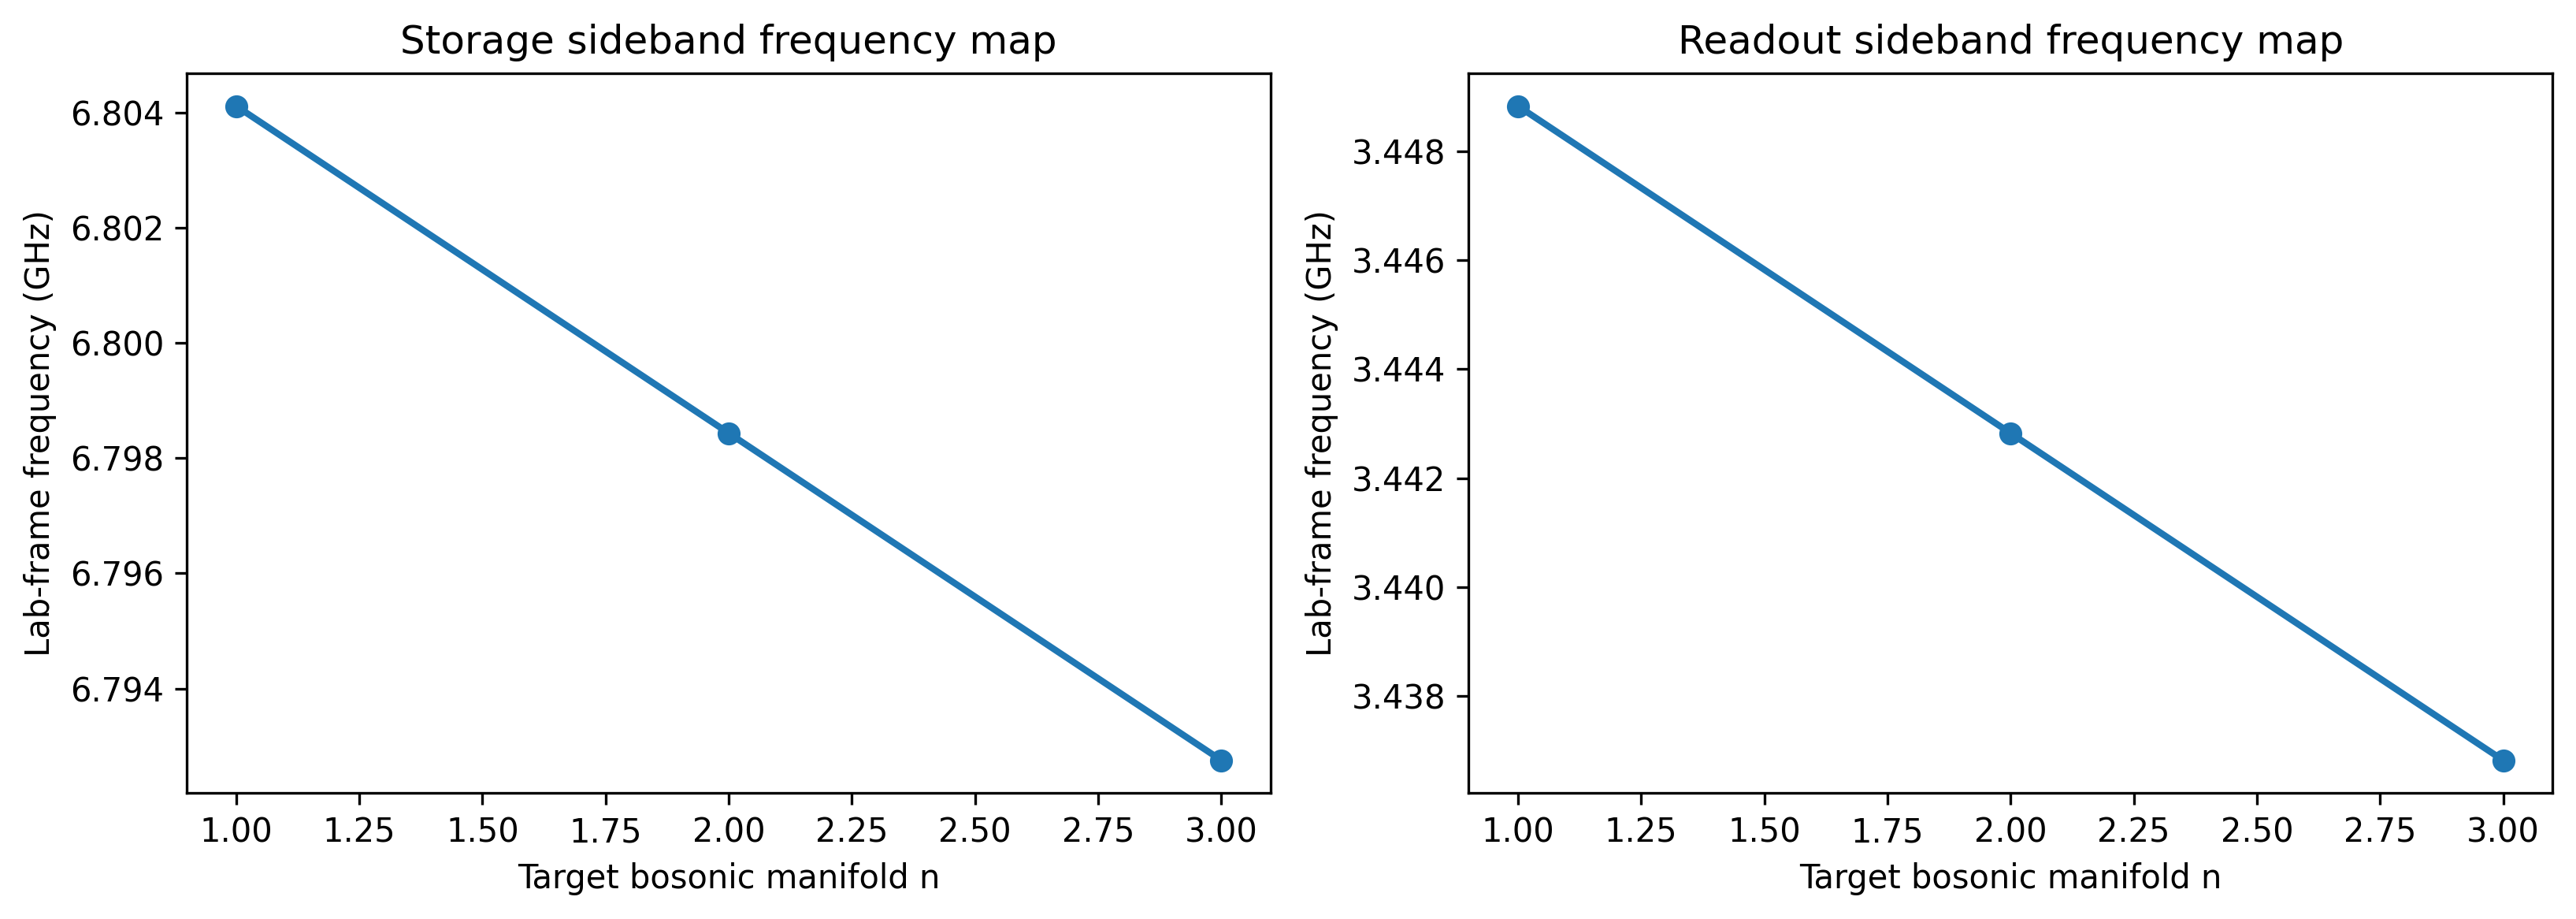
\includegraphics[width=0.9\linewidth]{../figures/sideband_frequency_map.png}
  \caption{Exact dressed sideband frequencies for the storage-mode and readout-mode interactions. The relevant same-mode line spacings are only a few megahertz, so short pulses are inevitably broad compared with the manifold spacing.}
  \label{fig:frequency_map}
\end{figure}

\begin{figure}[t]
  \centering
  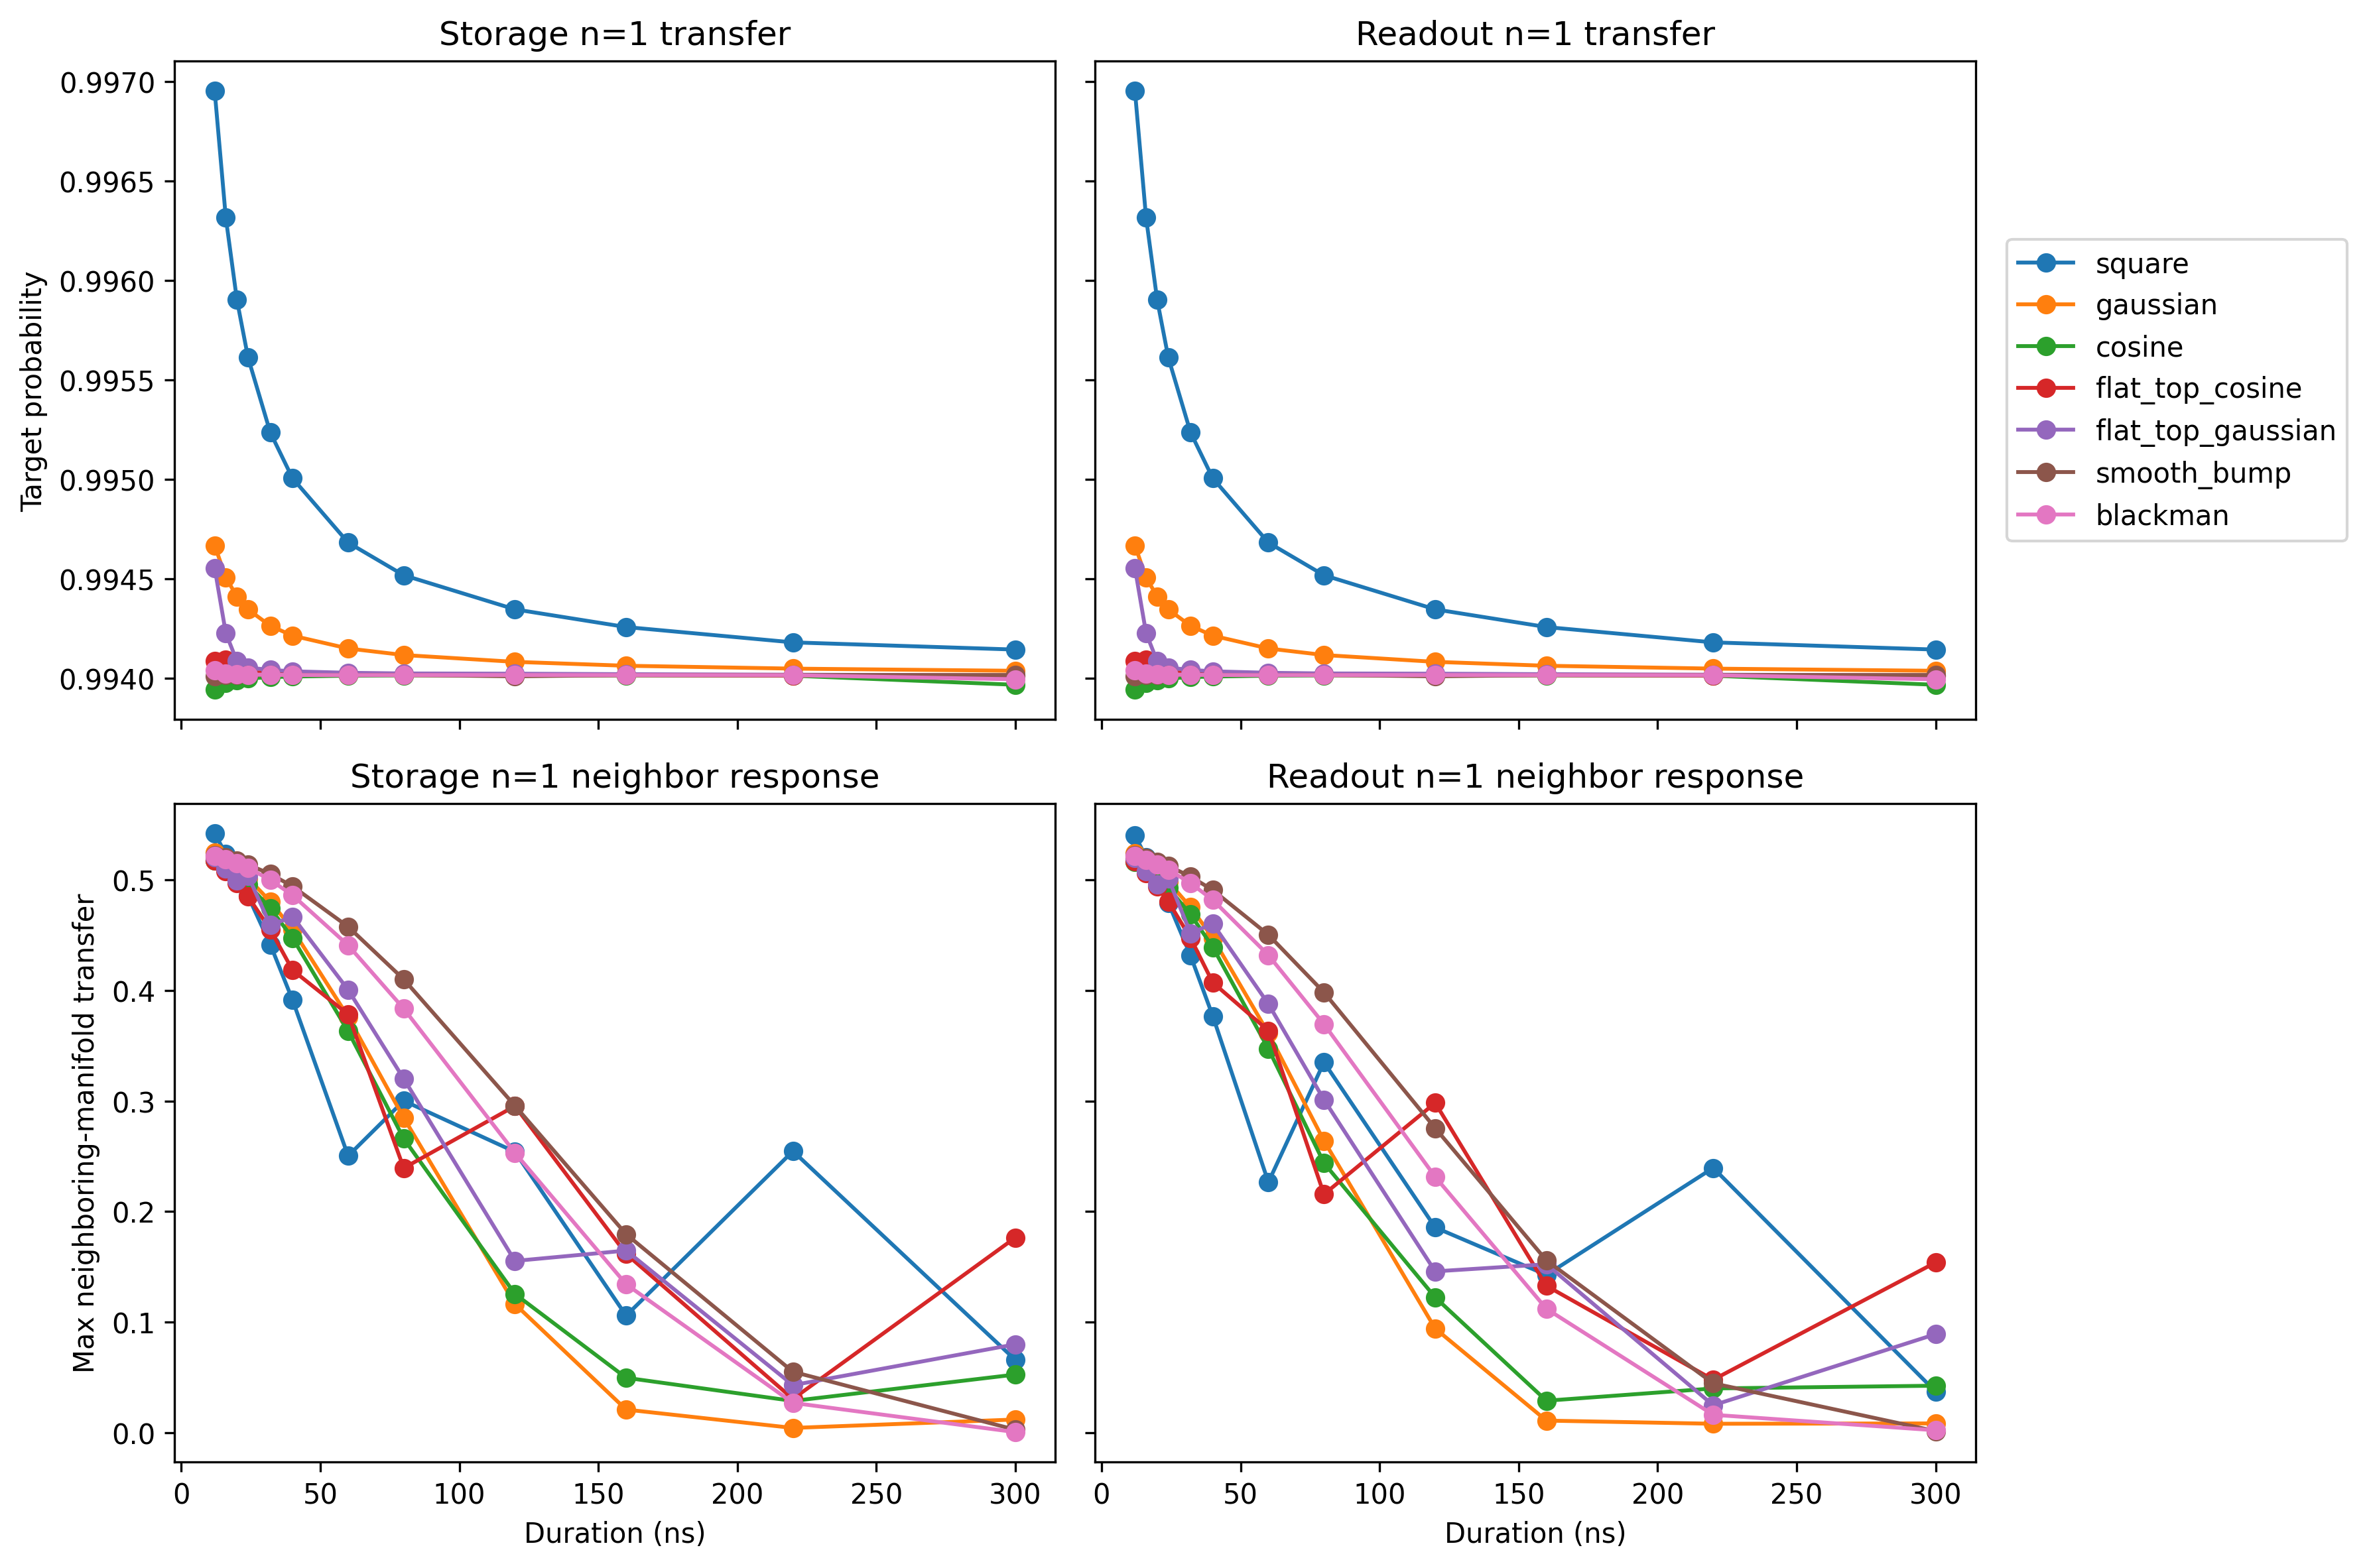
\includegraphics[width=\linewidth]{../figures/duration_tradeoff_n1.png}
  \caption{Representative \(n=1\) duration tradeoff. The main distinction between fast and selective control is the neighboring-manifold response, not the peak on-manifold transfer alone.}
  \label{fig:tradeoff}
\end{figure}

\begin{table}[t]
  \centering
  \caption{Closed-system family winners. Conservative duration means the smallest duration that works across \(n=1,2,3\) after amplitude retuning within the same family.}
  \label{tab:winners}
  \begin{tabular}{lllll}
    \toprule
    Mode & Regime & Family & Conservative duration & Mean target transfer \\
    \midrule
    Storage & Selective & Gaussian & \SI{300}{ns} & 0.99406 \\
    Storage & Fast unselective & Square & \SI{12}{ns} & 0.99695 \\
    Readout & Selective & Gaussian & \SI{220}{ns} & 0.99407 \\
    Readout & Fast unselective & Square & \SI{12}{ns} & 0.99696 \\
    \bottomrule
  \end{tabular}
\end{table}

The physical reason is the expected Fourier ranking. Square pulses maximize pulse area per unit time and therefore win whenever spectral discrimination is ignored. Wide Gaussian pulses suppress high-frequency spectral weight strongly enough to satisfy Eq.~\eqref{eq:selective_metric} across \(n=1,2,3\).

\begin{figure}[t]
  \centering
  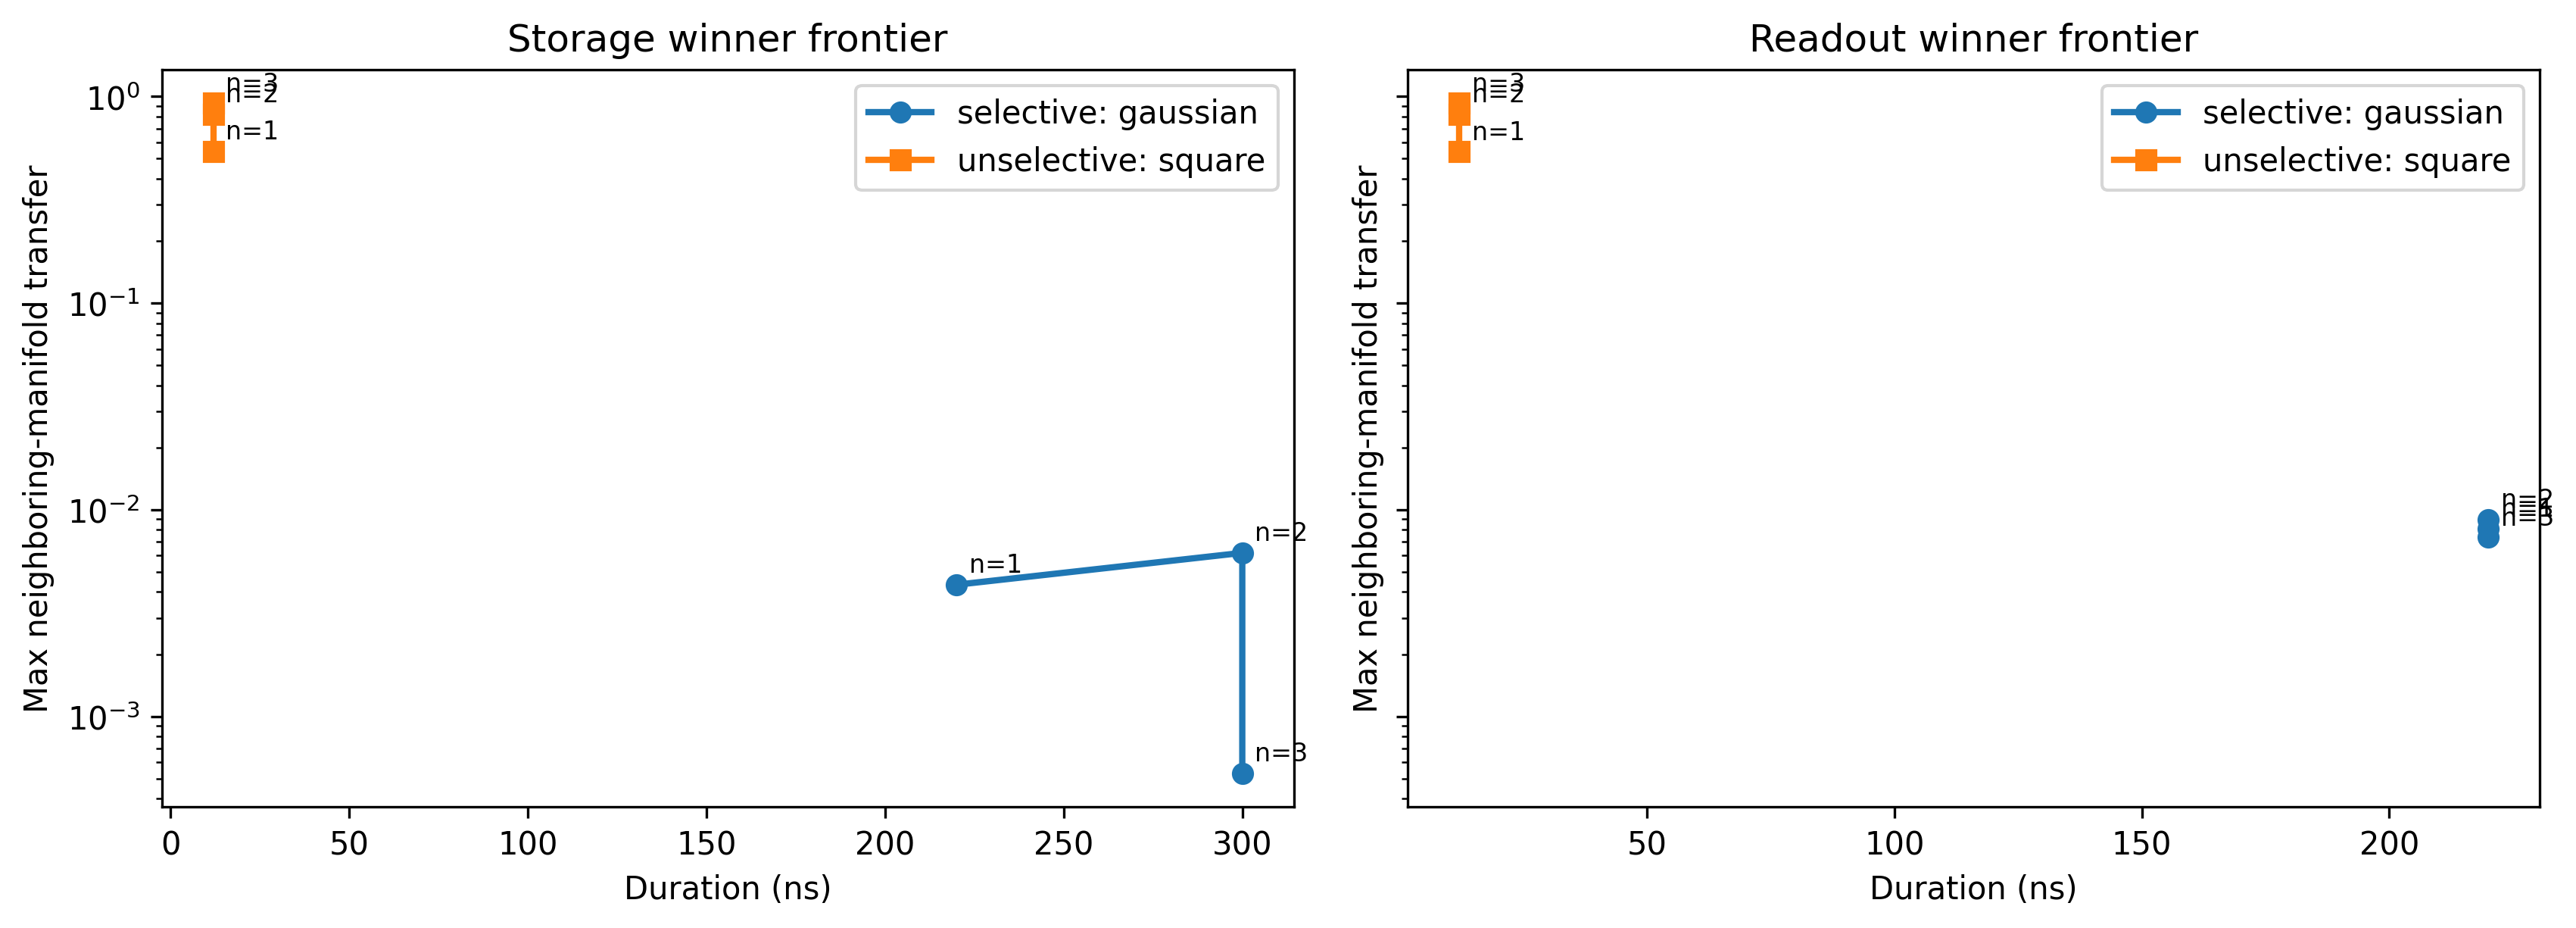
\includegraphics[width=0.92\linewidth]{../figures/winner_frontier.png}
  \caption{Winner frontiers for the two mode types. The selective Gaussian pulses occupy the long-duration, low-crosstalk corner, while the fast square pulses occupy the short-duration, high-crosstalk corner.}
  \label{fig:frontier}
\end{figure}

\subsection{Gate-Oriented Diagnostic}
The gate-oriented extension shows that the analytic family set is not producing a phase-clean SWAP gate even when transfer and leakage look excellent. Table~\ref{tab:gate} lists the best family under the gate-oriented diagnostic for each mode. The best mean projected SWAP fidelity reaches only \(0.716\) for storage and \(0.765\) for readout, with large residual phase asymmetry. The present winners should therefore be interpreted as state-transfer pulses rather than coherent gate solutions.

\begin{table}[t]
  \centering
  \small
  \caption{Best family under the gate-oriented diagnostic. These are still not uniformly phase-clean coherent SWAP gates across \(n=1,2,3\).}
  \label{tab:gate}
  \begin{tabular}{lcccc}
    \toprule
    Mode & Family & Duration & Mean projected fidelity & Mean phase asym. \\
    \midrule
    Storage & Gaussian & \SI{300}{ns} & 0.716 & 0.944 rad \\
    Readout & Blackman & \SI{300}{ns} & 0.765 & 0.839 rad \\
    \bottomrule
  \end{tabular}
\end{table}

\subsection{Open-System Results}
\subsection{Mode-Noise-Only Replay}
When only the dissipation channels exported directly by the sideband-reset example are included, the storage recommendations remain nearly unchanged while the readout selective regime collapses. The selective storage Gaussian retains mean target transfer \(0.99225\), whereas the selective readout Gaussian falls to \(0.33126\). The readout linewidth therefore already destroys the nominally selective \SI{220}{ns} readout pulse before any transmon decoherence is added.

\subsection{Including the Transmon Reference}
Table~\ref{tab:open_system} and Figure~\ref{fig:open_system} summarize the stronger open-system extension that includes the matched local transmon reference. The storage selective Gaussian remains the best \emph{structural} selective family, but its mean target transfer drops to \(0.96075\), so it no longer satisfies Eq.~\eqref{eq:selective_metric}. The fast storage square pulse remains above the fast-transfer threshold. The readout selective regime remains unusable, and the readout fast square pulse also falls below the original fast-transfer threshold once the full transmon-reference scenario is enforced.

\begin{table}[t]
  \centering
  \caption{Mean and worst-case target transfer for the closed-system winners under the matched transmon-reference noise scenario.}
  \label{tab:open_system}
  \begin{tabular}{llll}
    \toprule
    Mode & Regime & Mean noisy target & Worst noisy target \\
    \midrule
    Storage & Selective Gaussian & 0.96075 & 0.95655 \\
    Storage & Fast square & 0.99391 & 0.99385 \\
    Readout & Selective Gaussian & 0.32240 & 0.09952 \\
    Readout & Fast square & 0.92300 & 0.87740 \\
    \bottomrule
  \end{tabular}
\end{table}

\begin{figure}[t]
  \centering
  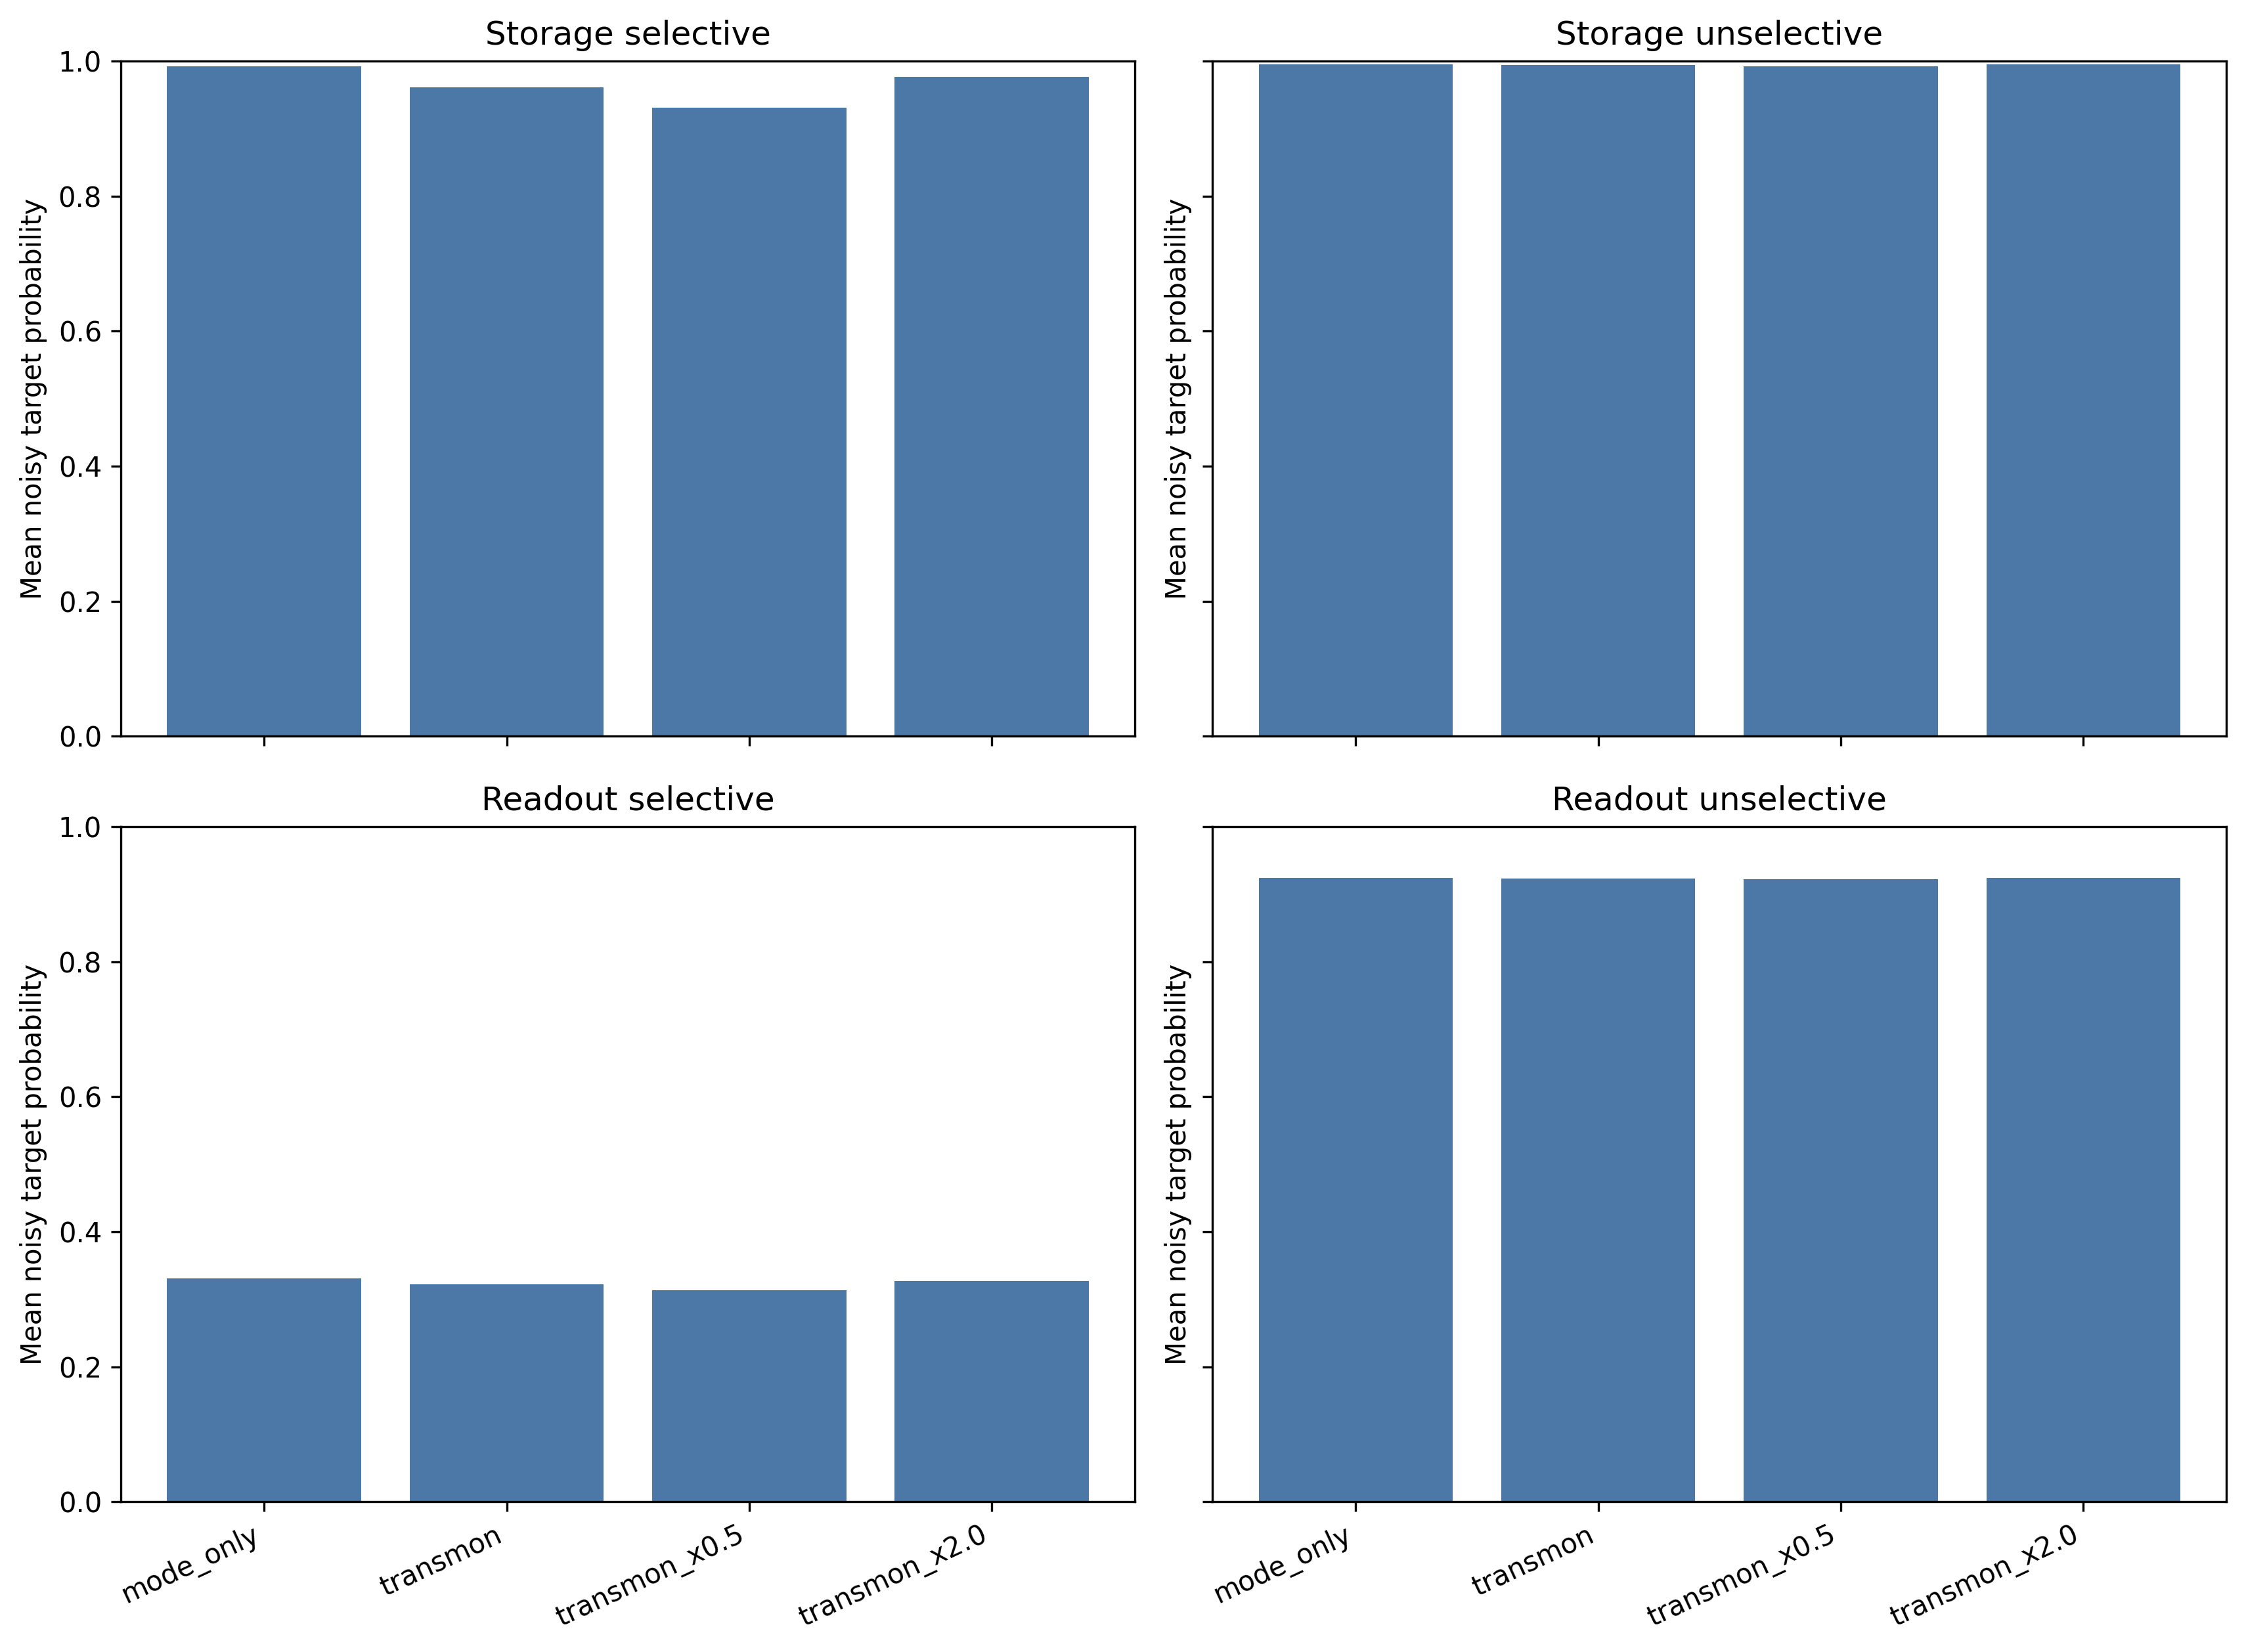
\includegraphics[width=\linewidth]{../figures/open_system_scenario_summary.png}
  \caption{Mean open-system target transfer across the noise scenarios. The readout selective regime fails in every noisy scenario, while the storage fast-square pulse is the only family that remains threshold-valid under the matched transmon-reference reranking.}
  \label{fig:open_system}
\end{figure}

The transmon-reference reranking is especially clear: only the storage fast-square family remains threshold-valid under the original metrics. No selective family survives, and no readout family survives.

\section{Validation}
Three validation checks were performed after the study extension. First, the exact rotating-frame sideband frequencies agree with Eqs.~\eqref{eq:storage_freq} and~\eqref{eq:readout_freq} to numerical precision for both modes and all \(n=1,2,3\). Second, finalist baselines use \SI{0.25}{ns} steps, and repeating them at \SI{0.5}{ns} changes the target transfer by only \(1.8\times 10^{-4}\) to \(1.4\times 10^{-3}\). Third, increasing the truncation from \((n_{\mathrm{tr}}, n_s, n_r)=(4,5,5)\) to \((5,6,6)\) changes finalist target transfer by at most \(5.7\times 10^{-5}\). The ranking is therefore stable with respect to the tested discretization and truncation changes.

\section{Discussion}
The closed-system control answer is simple: use a wide Gaussian for selective control and a square pulse for the fastest strong transfer. The experiment-facing answer is more conditional. If the only relevant open-system terms are the mode-noise channels exported directly by the sideband-reset example, storage selective control remains viable and readout selective control does not. Once the matched transmon-reference decoherence is included, the practical threshold-valid winner set collapses to a single family: the storage fast-square pulse. The same study therefore delivers both a control-theory ranking and a realism check on whether that ranking survives once coherence limits are imposed.

\section{Conclusion}
Within the effective sideband-control model, the waveform-ranking answer is consistent across both mode types: wide Gaussian pulses are best for selective transfer and square pulses are best for the fastest strong transfer. The practical open-system answer is much narrower: storage-sideband control remains useful, but selective readout-sideband control is not robust in the present linewidth regime, and only the storage fast-square pulse remains threshold-valid once the matched transmon-reference decoherence is included. The simultaneous two-tone extension further shows that a continuous resonant protocol can move a single storage photon into the readout mode on a \SI{29.5}{ns} timescale, but that benefit does not survive detuned slowing or generalize cleanly beyond the single-photon manifold.

\section{Limitations and Future Work}
The first limitation is model scope. The sideband is still represented as an effective control operator rather than as a microscopic pump Hamiltonian. The second limitation is parameter scope. The sideband-reset example does not export device-matched transmon \(T_1\) and \(T_2\), so the transmon-noise study is necessarily a matched local sensitivity analysis rather than a fully verified device model. The third limitation is objective scope. The gate-oriented extension adds a ranking diagnostic, but it does not perform direct unitary optimization. The most valuable next steps are therefore:
\begin{enumerate}
  \item introduce a microscopic pump-aware sideband model,
  \item add device-verified transmon coherence values on the exact sideband hardware instance,
  \item and optimize the projected two-state unitary directly when coherent gate use matters.
\end{enumerate}

\appendix
\section{Per-Manifold Closed-System Winner Parameters}
\begin{table}[H]
  \centering
  \caption{Per-manifold closed-system winner parameters.}
  \label{tab:appendix_winners}
  \begin{tabular}{llllrrr}
    \toprule
    Mode & Regime & \(n\) & Family & Duration (ns) & Amplitude (MHz) & Neighbor max \\
    \midrule
    Storage & Selective & 1 & Gaussian & 220 & 1.193 & 0.00434 \\
    Storage & Selective & 2 & Gaussian & 300 & 0.619 & 0.00619 \\
    Storage & Selective & 3 & Gaussian & 300 & 0.505 & 0.00053 \\
    Storage & Fast & 1 & Square & 12 & 21.875 & 0.54192 \\
    Storage & Fast & 2 & Square & 12 & 15.468 & 0.82029 \\
    Storage & Fast & 3 & Square & 12 & 12.630 & 0.92718 \\
    Readout & Selective & 1 & Gaussian & 220 & 1.193 & 0.00812 \\
    Readout & Selective & 2 & Gaussian & 220 & 0.844 & 0.00894 \\
    Readout & Selective & 3 & Gaussian & 220 & 0.689 & 0.00736 \\
    Readout & Fast & 1 & Square & 12 & 21.875 & 0.54028 \\
    Readout & Fast & 2 & Square & 12 & 15.468 & 0.81879 \\
    Readout & Fast & 3 & Square & 12 & 12.630 & 0.92542 \\
    \bottomrule
  \end{tabular}
\end{table}

\section{Transmon-Reference Threshold-Valid Winner Set}
Under the matched transmon-reference reranking, only one family remains threshold-valid under the original metrics:
\begin{center}
\begin{tabular}{llll}
\toprule
Mode & Regime & Family & Conservative duration \\
\midrule
Storage & Fast unselective & Square & \SI{12}{ns} \\
\bottomrule
\end{tabular}
\end{center}

\section{Saved Artifacts}
The saved machine-readable outputs include the parameter table, noise-scenario table, frequency table, coarse sweep, duration shortlist, duration-level metrics, selected cases, gate-oriented summaries, open-system summaries, transmon-reference reranking tables, robustness maps, trajectories, and the consolidated study summary. The figure set includes the frequency map, duration-tradeoff plot, winner frontier, representative dynamics, robustness maps, spectral-intuition comparison, and open-system scenario summary.

\clearpage
\section{Extension: Simultaneous Two-Tone Storage-to-Readout Transfer (Iteration 1)}
\label{sec:two_tone_extension}
This extension asks whether a continuous storage-sideband drive and a simultaneous readout-sideband drive can transfer a storage photon directly into the readout mode on the local device. For the single-photon manifold, the dominant reduced ladder is
\begin{equation}
|g,0,1\rangle \leftrightarrow |f,0,0\rangle \leftrightarrow |g,1,0\rangle,
\label{eq:two_tone_ladder}
\end{equation}
which is the minimal process that converts a storage photon into a readout photon through the transmon. Inside that ladder, the effective rotating-frame model is
\begin{equation}
\frac{H_{\mathrm{2tone}}}{\hbar} =
\begin{pmatrix}
0 & g_s & 0 \\
g_s & \Delta & g_r \\
0 & g_r & 0
\end{pmatrix},
\label{eq:two_tone_hamiltonian}
\end{equation}
where $g_s$ and $g_r$ are the storage-leg and readout-leg couplings and $\Delta$ is the common one-photon detuning of the intermediate state. Equation~\eqref{eq:two_tone_hamiltonian} makes the physical split between a resonant bright-state protocol ($\Delta=0$) and a detuned Raman-like protocol ($|\Delta| \gg g_s,g_r$) explicit.

\subsection{Single-Photon Mechanism and Performance}
Figure~\ref{fig:two_tone_scan} shows the closed-system scan over common detuning and target coupling. The resonant branch delivers the fastest transfer, while detuning suppresses the intermediate-state occupation at the price of a slower effective exchange. The best single-photon resonant case uses equal \SI{12}{MHz} leg couplings and reaches a peak target population of $0.9999977$ at \SI{29.5}{ns}. The best detuned single-photon case uses equal \SI{4}{MHz} leg couplings with a common detuning of \SI{20}{MHz}, reducing the peak intermediate-state population to $0.121$ but stretching the transfer to \SI{348}{ns}.

\begin{figure}[H]
  \centering
  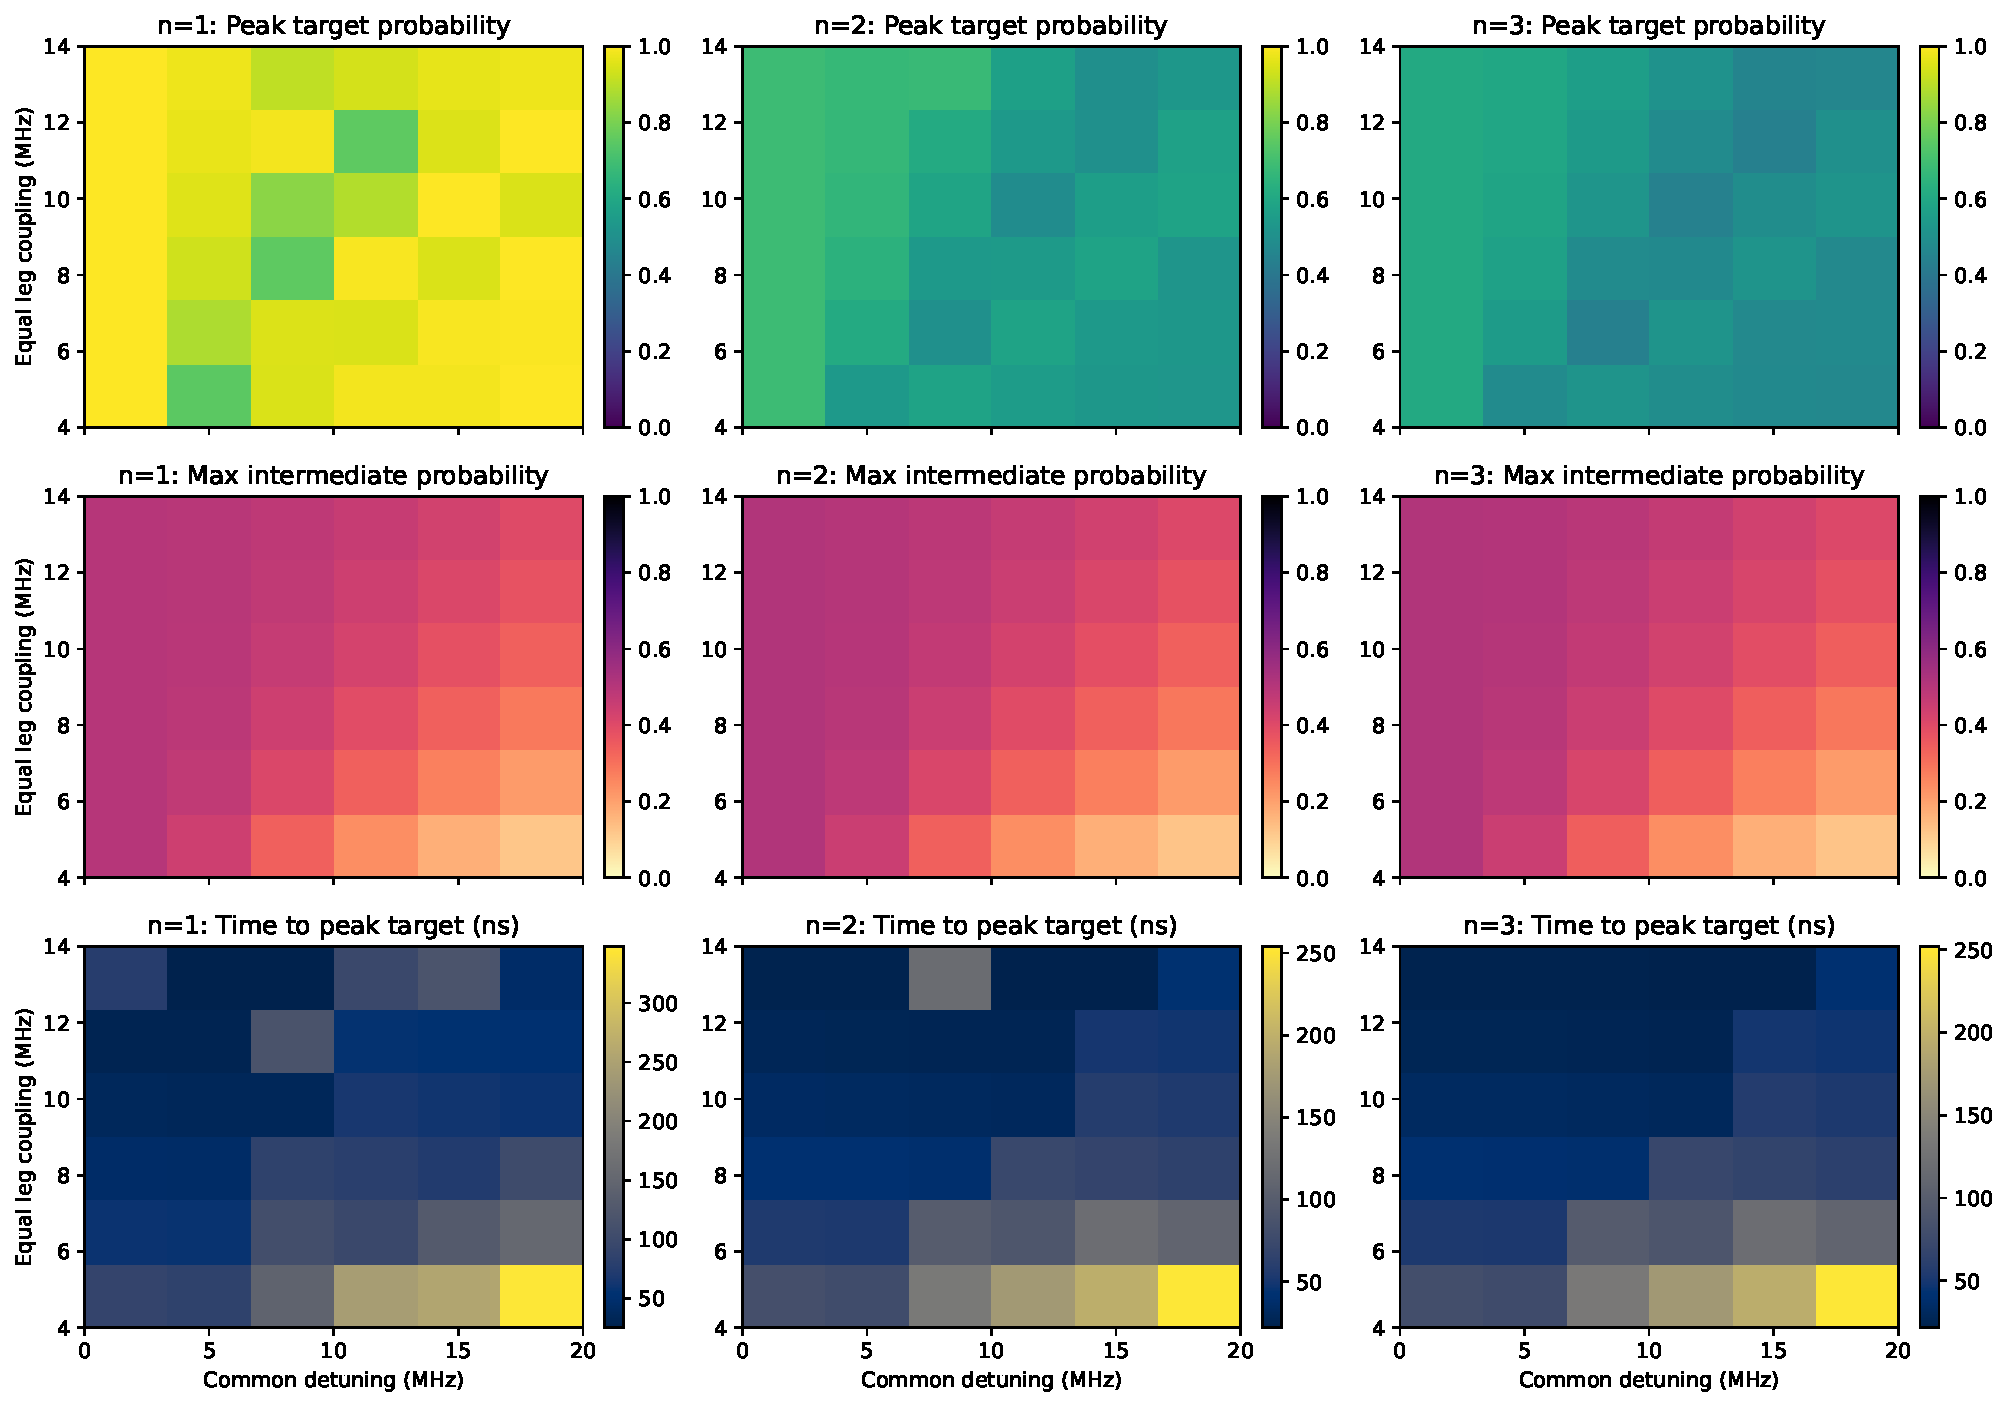
\includegraphics[width=\linewidth]{../figures/two_tone_scan_summary.pdf}
  \caption{Closed-system simultaneous two-tone scan summary. The single-photon resonant region reaches near-unit transfer on a \SI{10}{ns}-scale, whereas the detuned Raman-like region lowers intermediate-state occupation at the price of much longer transfer times.}
  \label{fig:two_tone_scan}
\end{figure}

Figure~\ref{fig:two_tone_dynamics} compares the selected resonant and detuned cases. For $n=1$, the full simulator agrees closely with the reduced model from Eq.~\eqref{eq:two_tone_hamiltonian}: the resonant selected case matches the reduced-model peak target probability to within $4.1\times 10^{-7}$ and reproduces the peak time exactly. The same figure also shows why the higher-photon cases do not generalize cleanly. For $n>1$, the constant simultaneous drive opens a longer conversion chain, so the reduced three-state picture from Eq.~\eqref{eq:two_tone_ladder} no longer captures the dynamics and the best resonant target population stalls near $0.61$--$0.69$ even without noise.

\begin{figure}[H]
  \centering
  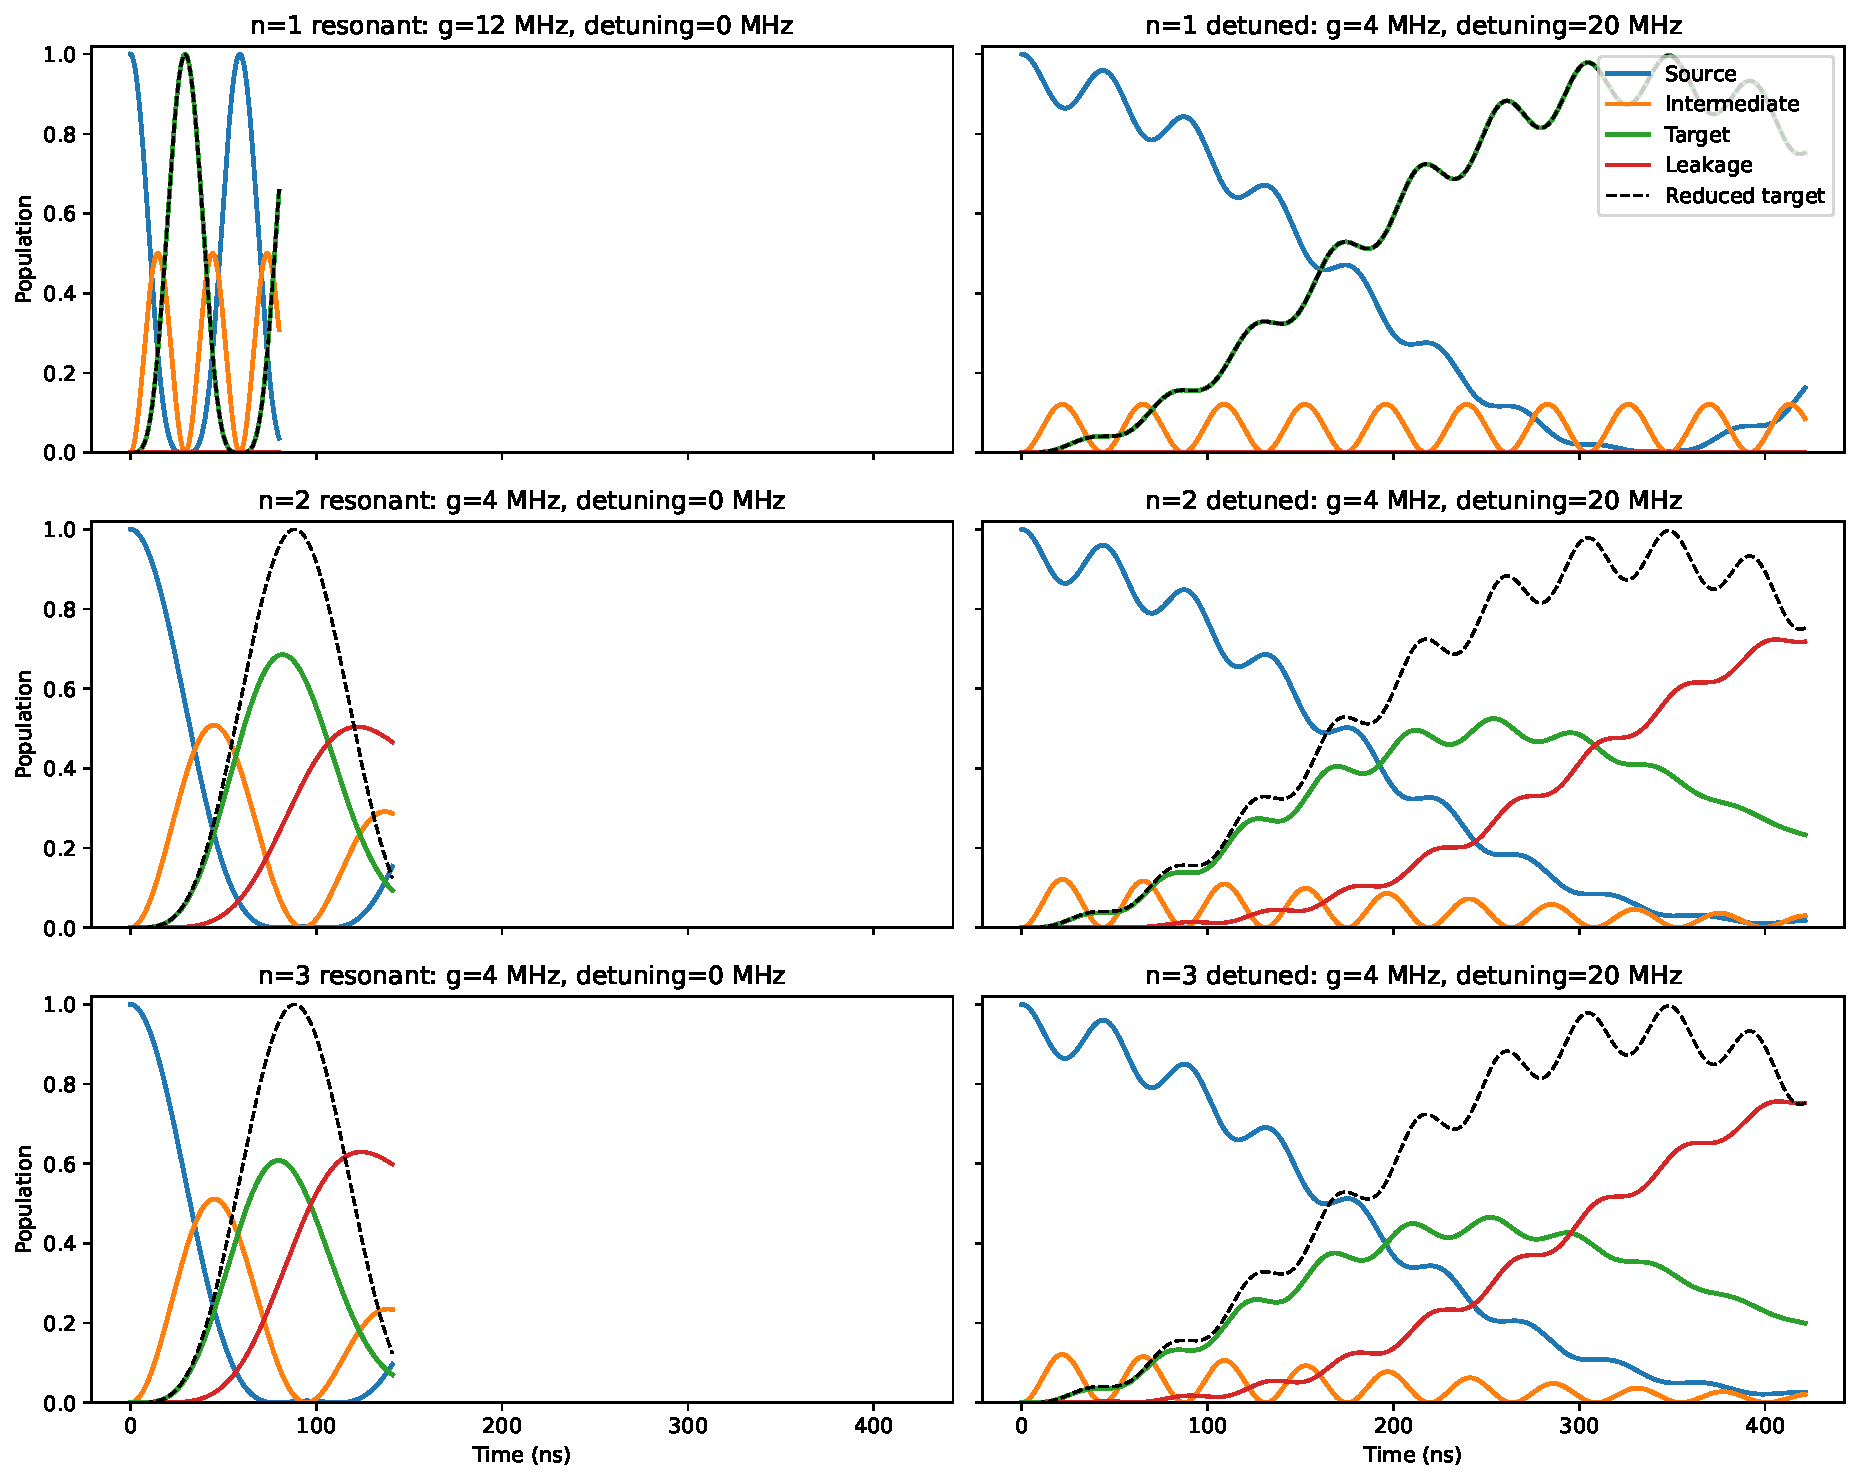
\includegraphics[width=\linewidth]{../figures/two_tone_population_dynamics.pdf}
  \caption{Population dynamics for the selected simultaneous two-tone cases. The single-photon resonant and detuned cases closely follow the reduced ladder model, while the $n=2$ and $n=3$ cases visibly depart from that picture because the continuous drive couples into a longer conversion chain.}
  \label{fig:two_tone_dynamics}
\end{figure}

\subsection{Open-System Viability}
The open-system replay in Table~\ref{tab:two_tone_open} and Figure~\ref{fig:two_tone_open} shows that the resonant single-photon protocol remains viable under the local noise model, whereas the slower detuned protocol does not. With mode noise only, the resonant case peaks at $0.9554$ and the matched transmon-reference replay gives $0.9530$, both at \SI{29.25}{ns}. The detuned case peaks at only $0.5606$ with mode noise and $0.5560$ with the transmon reference, because the readout linewidth drains the target mode before the slower Raman-like transfer can complete.

\begin{table}[H]
  \centering
  \caption{Selected single-photon simultaneous two-tone cases in the closed and open systems.}
  \label{tab:two_tone_open}
  \begin{tabular}{lcccc}
    \toprule
    Case & Closed peak & Peak time & Mode-noise peak & Transmon-ref. peak \\
    \midrule
    Resonant bright state & 0.9999977 & \SI{29.5}{ns} & 0.9554 & 0.9530 \\
    Detuned Raman-like & 0.99677 & \SI{348.0}{ns} & 0.5606 & 0.5560 \\
    \bottomrule
  \end{tabular}
\end{table}

\begin{figure}[H]
  \centering
  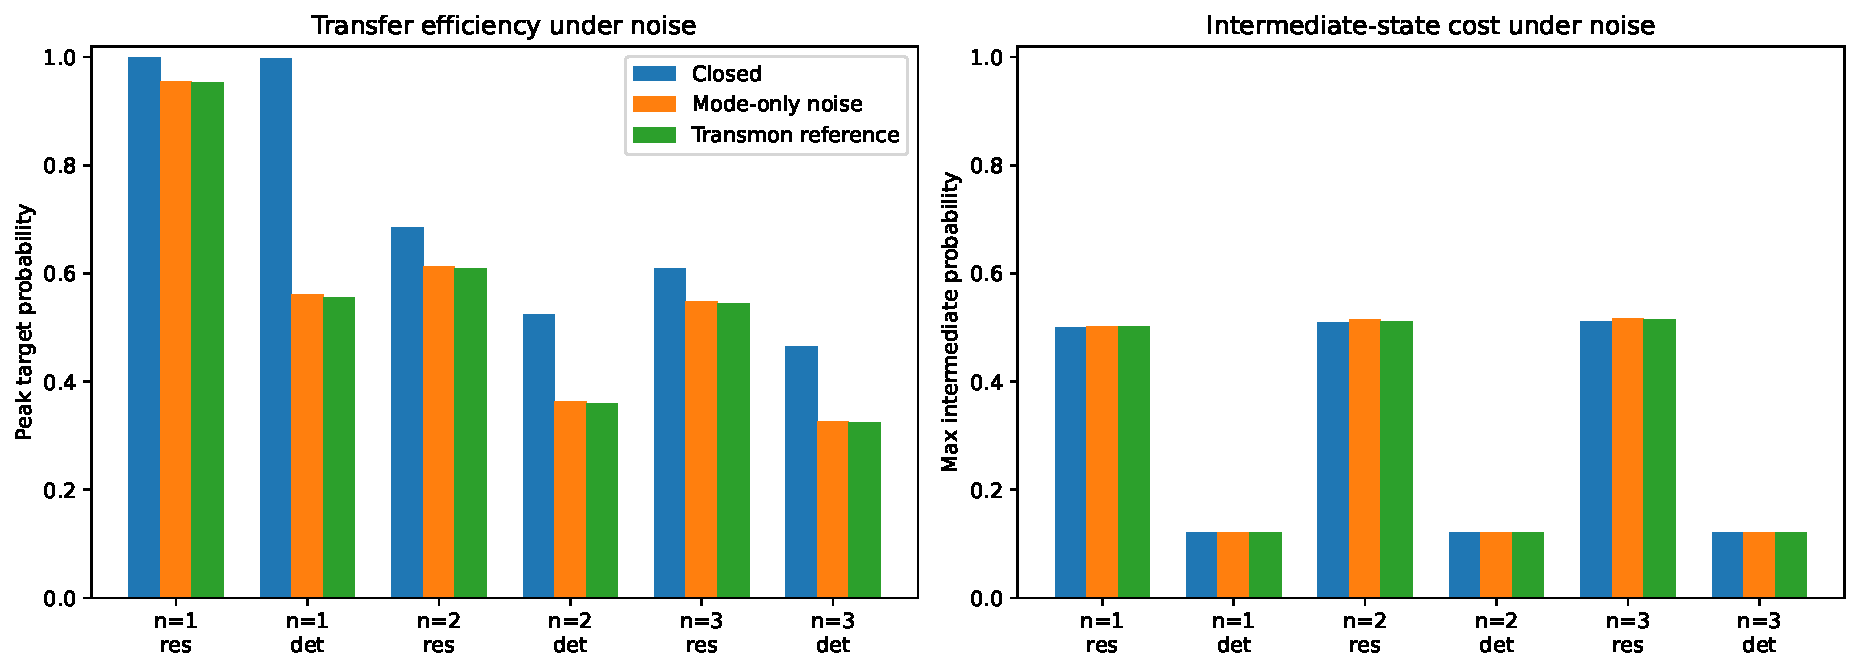
\includegraphics[width=0.9\linewidth]{../figures/two_tone_open_system_summary.pdf}
  \caption{Open-system summary for the selected simultaneous two-tone cases. The fast resonant single-photon protocol survives the available decoherence much better than the slower detuned Raman-like protocol.}
  \label{fig:two_tone_open}
\end{figure}

The practical conclusion is therefore narrower than the closed-system intuition alone would suggest. A continuous simultaneous two-tone drive is a plausible fast single-photon storage-to-readout transfer primitive on this device if large transient intermediate-state occupation is acceptable. The detuned constant-drive variant is not competitive in the same hardware regime, and the protocol should not be extrapolated to arbitrary storage Fock states without adding number-selective structure or shaped counter-intuitive overlap.

\end{document}
